\chapter{Technical Background}
This chapter describe briefly the different building blocks to do deep learning models, the metrics to evaluate them once trained and how the output of a model can be explained.

\section{Model blocks}

\subsection{Fully Connected}

One of the most basic component when building a Deep Learning model is the fully connected (FC) layer. Mathematically it is defined as:
$$Y=X*W + b$$
Where $Y$ the outputs are express as a linear combination of the inputs $X$ and a bias $b$. It has been proven by the well know \textbf{Universal approximation theorem} that such layers combine with non linear functions can approximate in theory any continuous functions.

\subsection{3D CNN}

\begin{wrapfigure}{r}{0.6\textwidth}
 \centering
 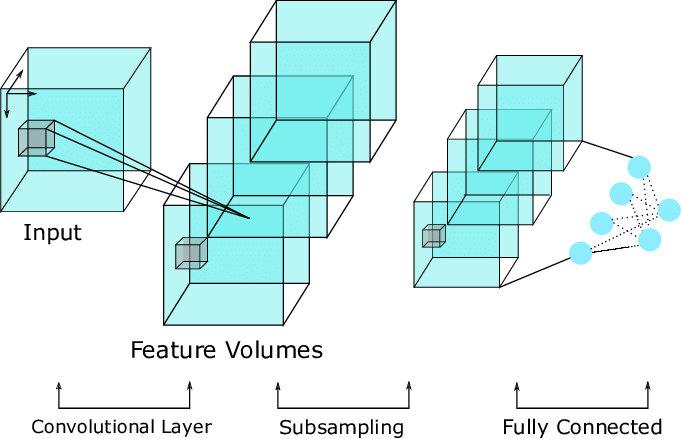
\includegraphics[width=.9\linewidth]{figures/3D_CNN_example.png}
 \captionsetup{width=.9\linewidth}
 \caption[3D_CNN_example]{Illustration\footnotemark{} of a 3D CNN Network}
 \label{fig:3d_cnn_example}
\end{wrapfigure}
\footnotetext{\href{https://www.researchgate.net/publication/330912338_ECNN_Activity_Recognition_Using_Ensembled_Convolutional_Neural_Networks}{https://www.researchgate.net/publication/330912338\_ECNN\_Activity\_Recognition\_Using\_Ensembled\_Convolutional\_Neural\_Networks}}
The fully connected layer presented above are really general and work well with a large variety of data as no assumption is made. Unfortunately, for certain kind of data it can quickly become unscalable to use a FC layers. For example, when dealing with images of size 200 by 200 in color, a layer with 100 features output would already required 12'000'100 parameters to be learned (including bias).

One of the assumption that convolutional layers makes when dealing with images, is spacial locality. Pixels close to each other are more likely to be correlated that distant ones. From this assumption, CNN can be seen as small FC layer that are apply at multiple location across the image. Those one are usually call kernel. 

This way of computing the inputs does have multiple advantages. One of the them being weight sharing. The kernel being apply at multiple location, the weight learned to extract a feature in one location are by construction reused to extract the same features everywhere else in the image. Another property of CNN that comes directly from how it is computed is translation equivariance. Now a day, CNN have become the standard way of treating image.

In our case, the MRI which are 3D images, are even larger that standard image and therefore for all the same reason why you want to use a CNN to process a 2D image, it makes even more sense to use a 3D CNN when dealing with 3D image. The only difference you get between 2D CNN and 3D CNN is the shape of the kernel you are learning, which are now 3D as the input. Figure \ref{fig:3d_cnn_example} illustrate how similar 3D CNN are to 2D CNN.



\section{Losses and Metrics}
\label{sec:losses_metrics}
This section list the different metrics and loss used during that project.

\subsection{Binary Cross Entropy}
\label{sec:binary_cross_entropy}

$$ L = -(y\log(p) + (1-y)\log(1-p))$$

\subsection{Mean Square Error (MSE)}
\label{sec:mean_square_error}
This loss is used to penalize errors done by a network for example in the case of a regression. It works with continues values and is defined as:
$$ MSE = \frac{\sum_{i=1}^{n} (Y_i - \^{Y}_i)^2}{n}$$
Where $\^{Y}_i$ is the predicted value and $Y_i$ is the target value.
\subsection{Mean Absolute Error (MAE)}
This metrics is really similar to the MSE, but we take the absolute value of the error instead of raising it to the square.
$$ MAE = \frac{\sum_{i=1}^{n} |(Y_i - \^{Y}_i)|}{n}$$
\subsection{Accuracy}
The accuracy is one of the simplest metrics to evaluate a model. It is computed by counting the number of correctly classified sampled divided by the total number of sample.


\subsection{Precision and Recall}
While accuracy is simple to understand and to visualise, it can often fail at evaluating the performance of a model when the dataset is unbalanced with regards to the classes. To overcome that issue other metrics can be computed based on the true/false positive and true/false negative.

\begin{itemize}
    \item \textbf{True positive (TP)}: Positive sample correctly classified as positive. 
    \item \textbf{False positive (FP)}: Negative sample badly classified as positive. 
    \item \textbf{True negative (TN)}: Negative sample correctly classified as negative. 
    \item \textbf{False negative (FN)}: Positive sample badly classified as negative.
\end{itemize}

Precision can thus be computed as bellow and give a sense on how precise you are with your prediction.
$$Precision = \frac{TP}{TP +  FP}$$

Recall on the other hands can be computed as bellow and gives a sense on how likely the model is to detect dementia when the patient is really dement.
$$Recall =\frac{TP}{TP + FN}$$
In medical situation it might be more interesting to have a model with a good recall at the expense of precision. The consequences of being detected as healthy when in fact you suffer from the disease is often worst than the opposite. 

It turns out that accuracy can also be computed with those terms.


$$Accuracy = \frac{TP + TN}{TP + TN + FP + FN}$$


\subsection{ROC - AUC}
Receiver Operating Characteristic allows for plotting a chart like figure \ref{fig:roc_curve} that visualize the precision and recall at different threshold. From that curve we can compute the Area Under the Curve (AUC) which is a good metric to compare different model. Usually a bigger AUC means a better model, but what one is really interested into is how fast the curve is raising. 
In an ideal situation we expect the curve to touch the top left corner and have an AUC of 1.

\subsection{PR - Curve}
The Precision and Recall is often use in replacement of the ROC curve when dealing with unbalanced data. TODO.


\section{Transfer learning with Auto-Encoder}
Autoencoders are a class of neural network, usually used to encode the data into a latent space. The idea is quite simple, the network is made of two components, an \textit{encoder}, which maps the original data to the latent space and a \textit{generator} which maps back from the latent space to the original space of the data. Note that the latent space must be of lower cardinality than the input, otherwise th encoder could simply learn the identity function. The training goal is to reconstruct as accurately as possible the the input data. To ensure that, the loss used can be either mean square error with no activation to the last layer. If the input data has been normalized into the range $[0, 1]$, by applying a $sigmoid$ function to the the last layer one could use the binary cross entropy loss as an alternative, though the lost won’t converge to zero. 

The loss is comparing the input data with the network output, thus making this kind of neural network fall into the network that can be trained in an unsupervised manner. This is especially interesting when you have a problem with a lot of data but only a few of them are labeled. The Autoencoders can be an easy solution to extract interesting features from the dataset not related to any task. The weights learned during the training can be later reused in combination with another network to either classify or do any related supervised task.

Another similar network is the denoising Autoencoder \cite{denoising_autoencoder_10.5555/1756006.1953039}. It is trained to remove artificially added noise to from its inputs. It as the advantage of not requiring a compression of the input in dimension and is also know to extract better features.

This model has been implemented, but as we did not get much unlabeled data either, we did not see any improvement it.

\section{Model Explication}
There exist different way to explain the output of a model. We tried different approach that either are specific to computer vision task or more general and compare them for our specific task of dementia prediction.

\subsection{Shap}
Shap is an algorithm based on Game Theory that aimed to predict the contribution of a feature to increase the confidence of a model. It’s mathematical background lies on the shapley value which basically is the average of the marginal contribution across all permutation of the features.

\begin{wrapfigure}{l}{0.7\textwidth}
 \centering
 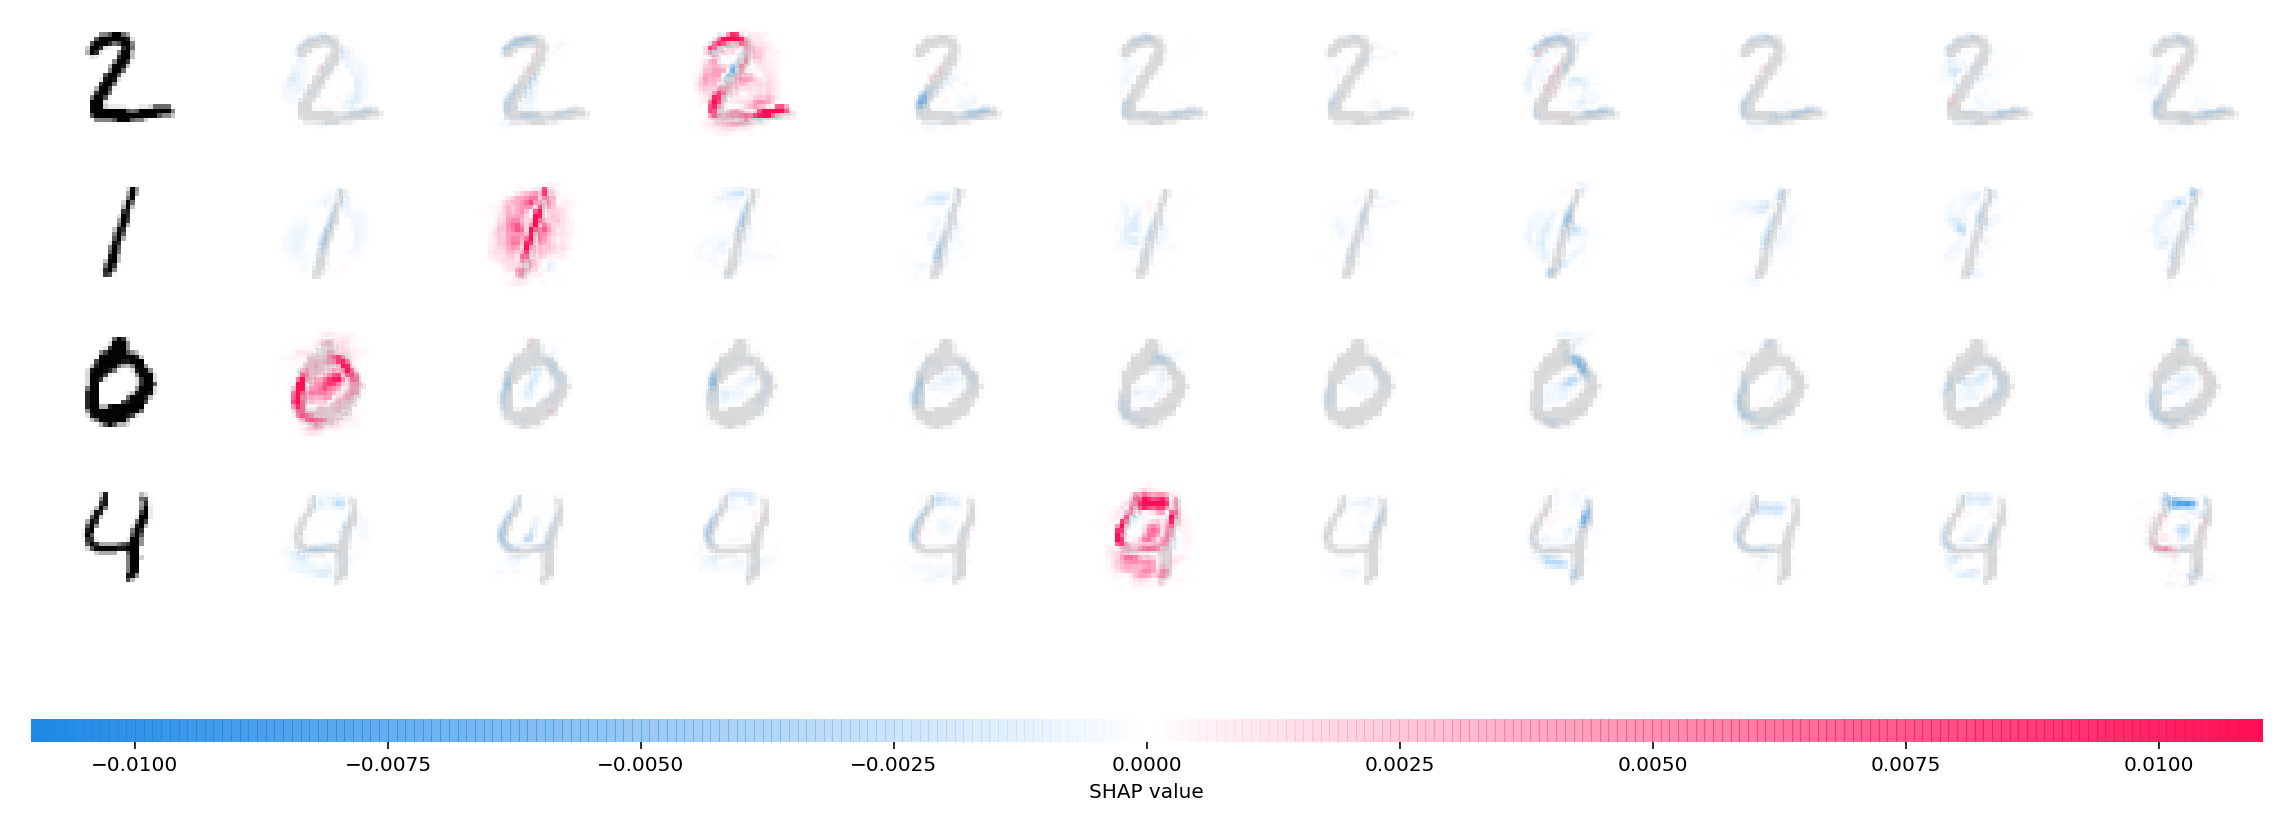
\includegraphics[width=.9\linewidth]{figures/shap_mnist_image_plot.png}
 \captionsetup{width=.9\linewidth}
 \caption[ShapExample]{Example of shap value from the Shap repo\footnotemark{}. Each column represent the shap output for a specific class (in a sorted order).}
 \label{fig:shap_example}
\end{wrapfigure}
\footnotetext{\href{https://github.com/slundberg/shap}{https://github.com/slundberg/shap}}

The library\cite{shap_lundberg2017unified} works with different kinds of models but it was tested with the GradientExplainer as DeepExplainer is not fully compatible with Pytorch yet. Compared to some other explainer algorithm, Shap presents the advantage of giving negative value for a feature which has a negative correlation with the output. The output obtained by that process can be seen in figure\ref{fig:explainer_compared}, but we can see that it does not give good interpretation incredible in comparison with other techniques.



\subsection{Grad-Cam}
When the input is an image, people are interesting into finding which part of the image better explain the prediction. In his paper\cite{zhou2015cnnlocalization} Zhou, propose a specific model for which he could create a \textit{class activation maps}. This idea has been generalized to work with any model by the authors of grad-cam. 

\begin{figure}
    \centering
    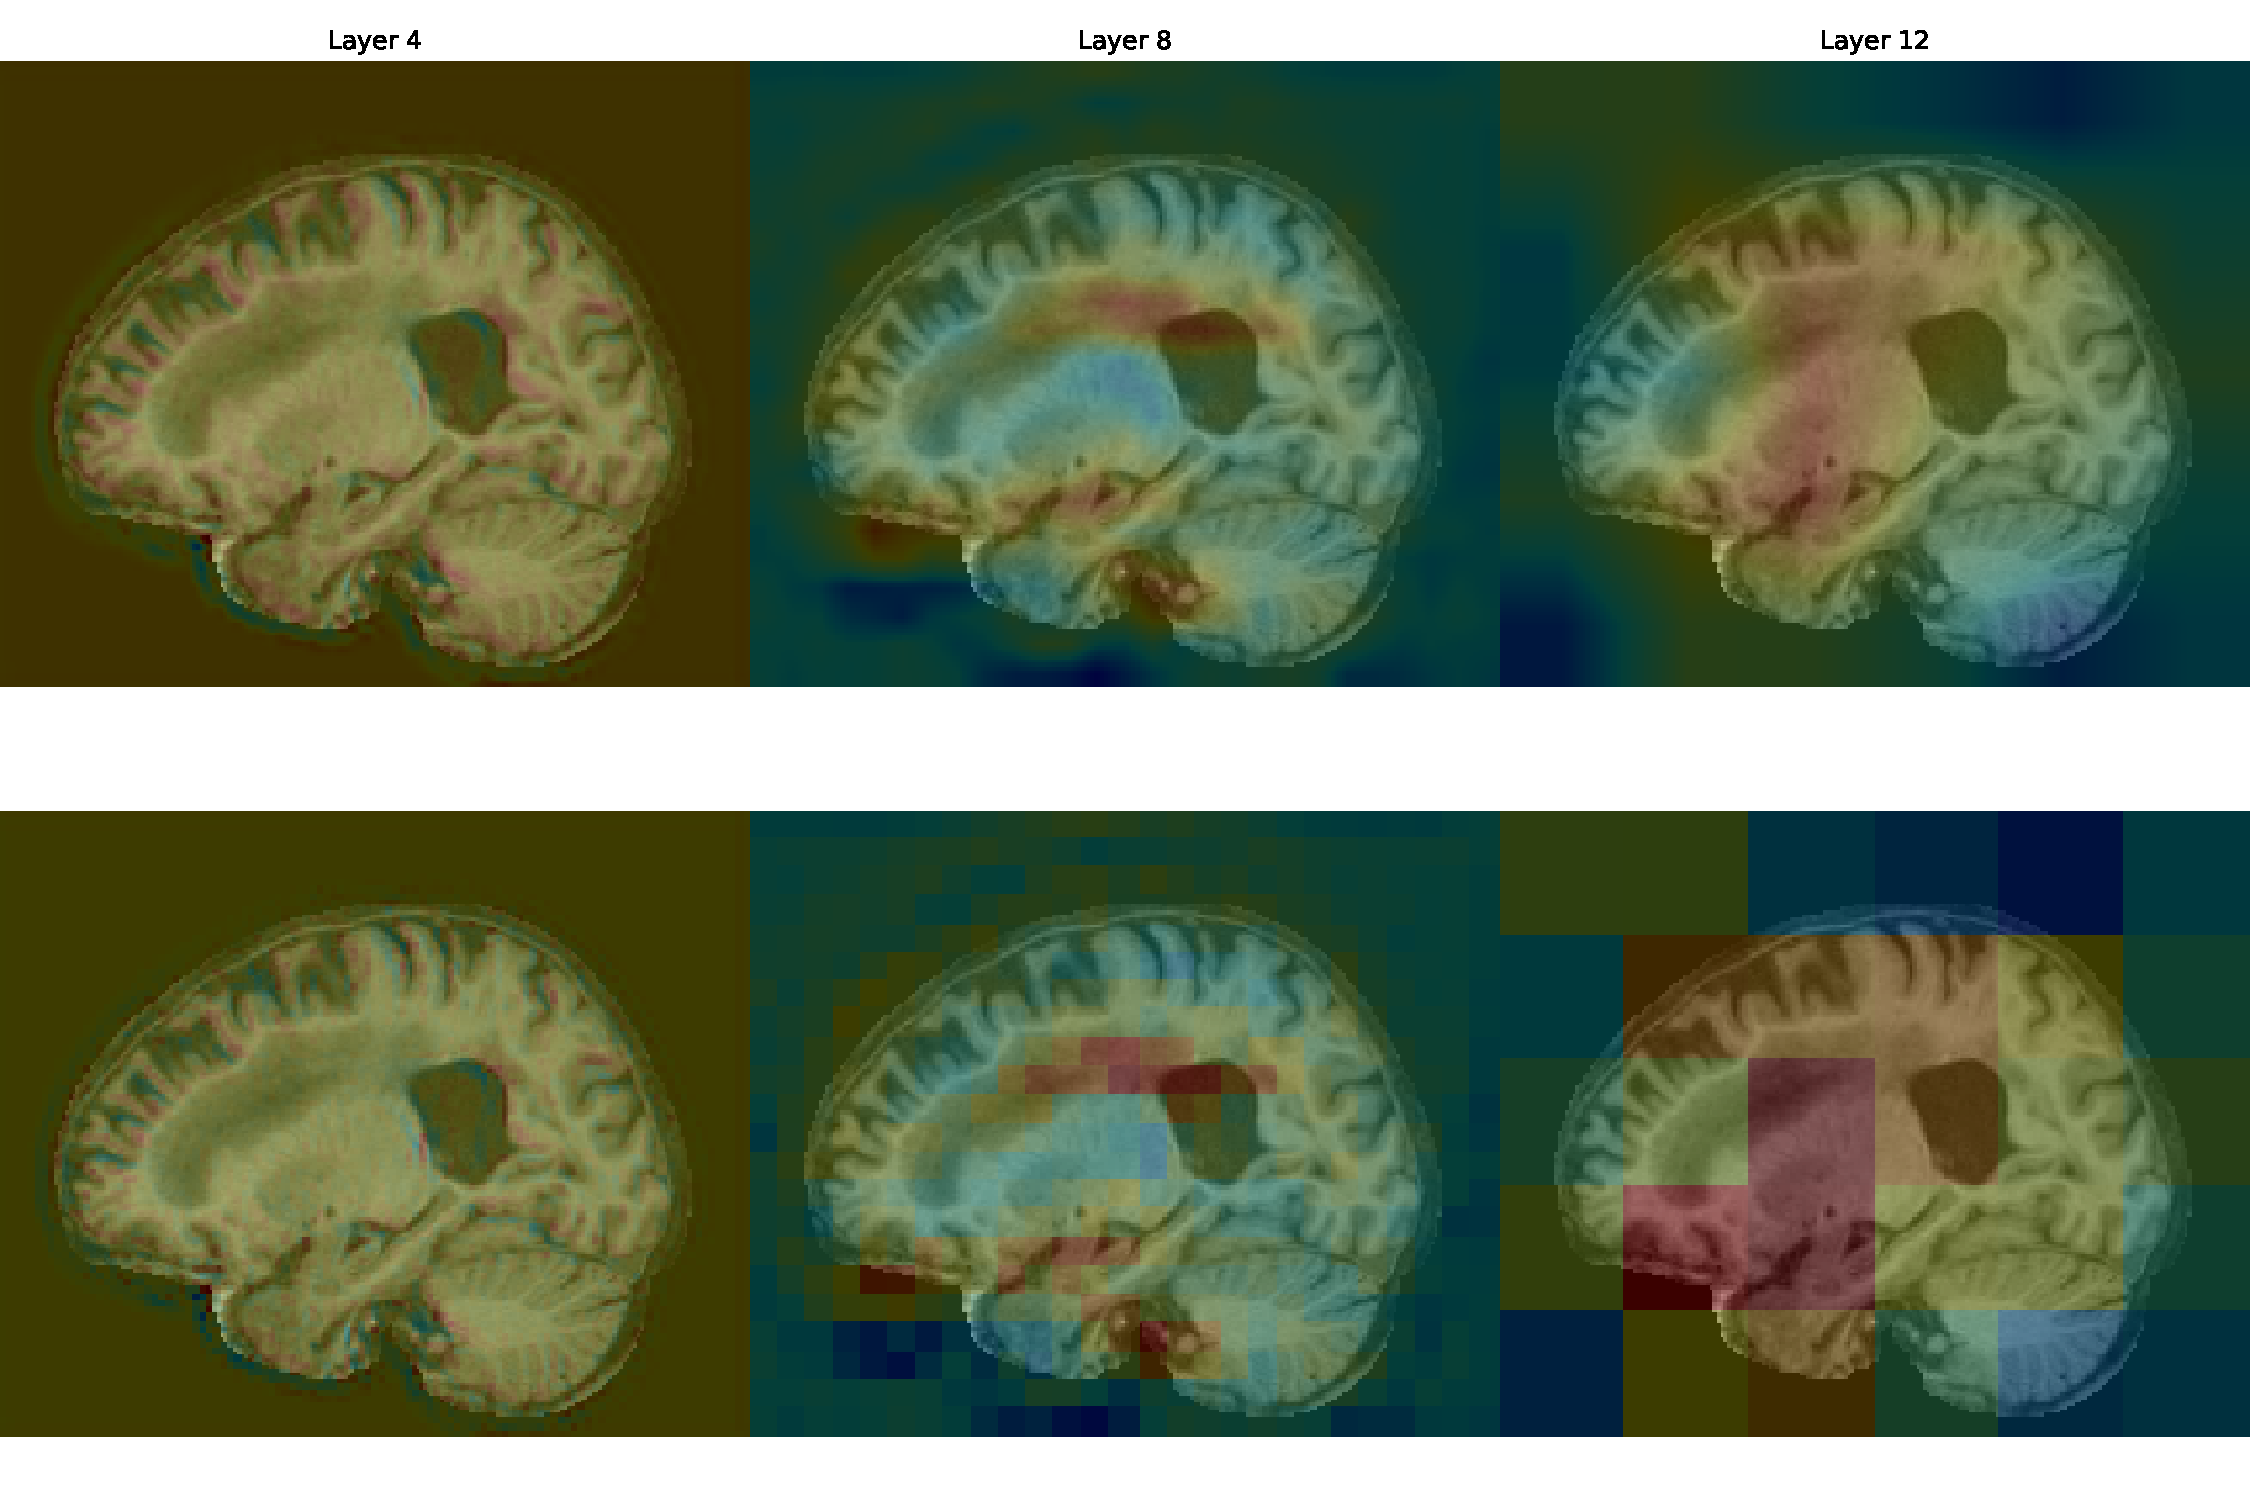
\includegraphics[width=400]{figures/gradcam_multilayer.pdf}
    \caption{GradCam saliency map seen at different layer. Trilinear interpolation is used in first row and nearest interpolation in second row.}
    \label{fig:grad_cam_multilayer}
\end{figure}

The Grad-Cam\cite{grad_cam_2019} algorithm is looking for activation of the neurons at a particular layer. To do so the input is processed in a forward pass by the network until the final prediction is done. The gradient of the predicted class with respect to the layer of interest is then computed. It is then pool across its spatial dimension in order to get a value of layer importance per channel. The features extracted from the image are then multiplied channel wised by the pooled gradient in order to get an activation map (also called saliency map) of the same shape at the output of the layer of interest. This can be map to the original image shape by interpolation. For visual purposes we choose to do a trilinear interpolation. This algorithm is well schematized in figure \ref{fig:grad_cam_arch}.

\begin{figure}
    \centering
    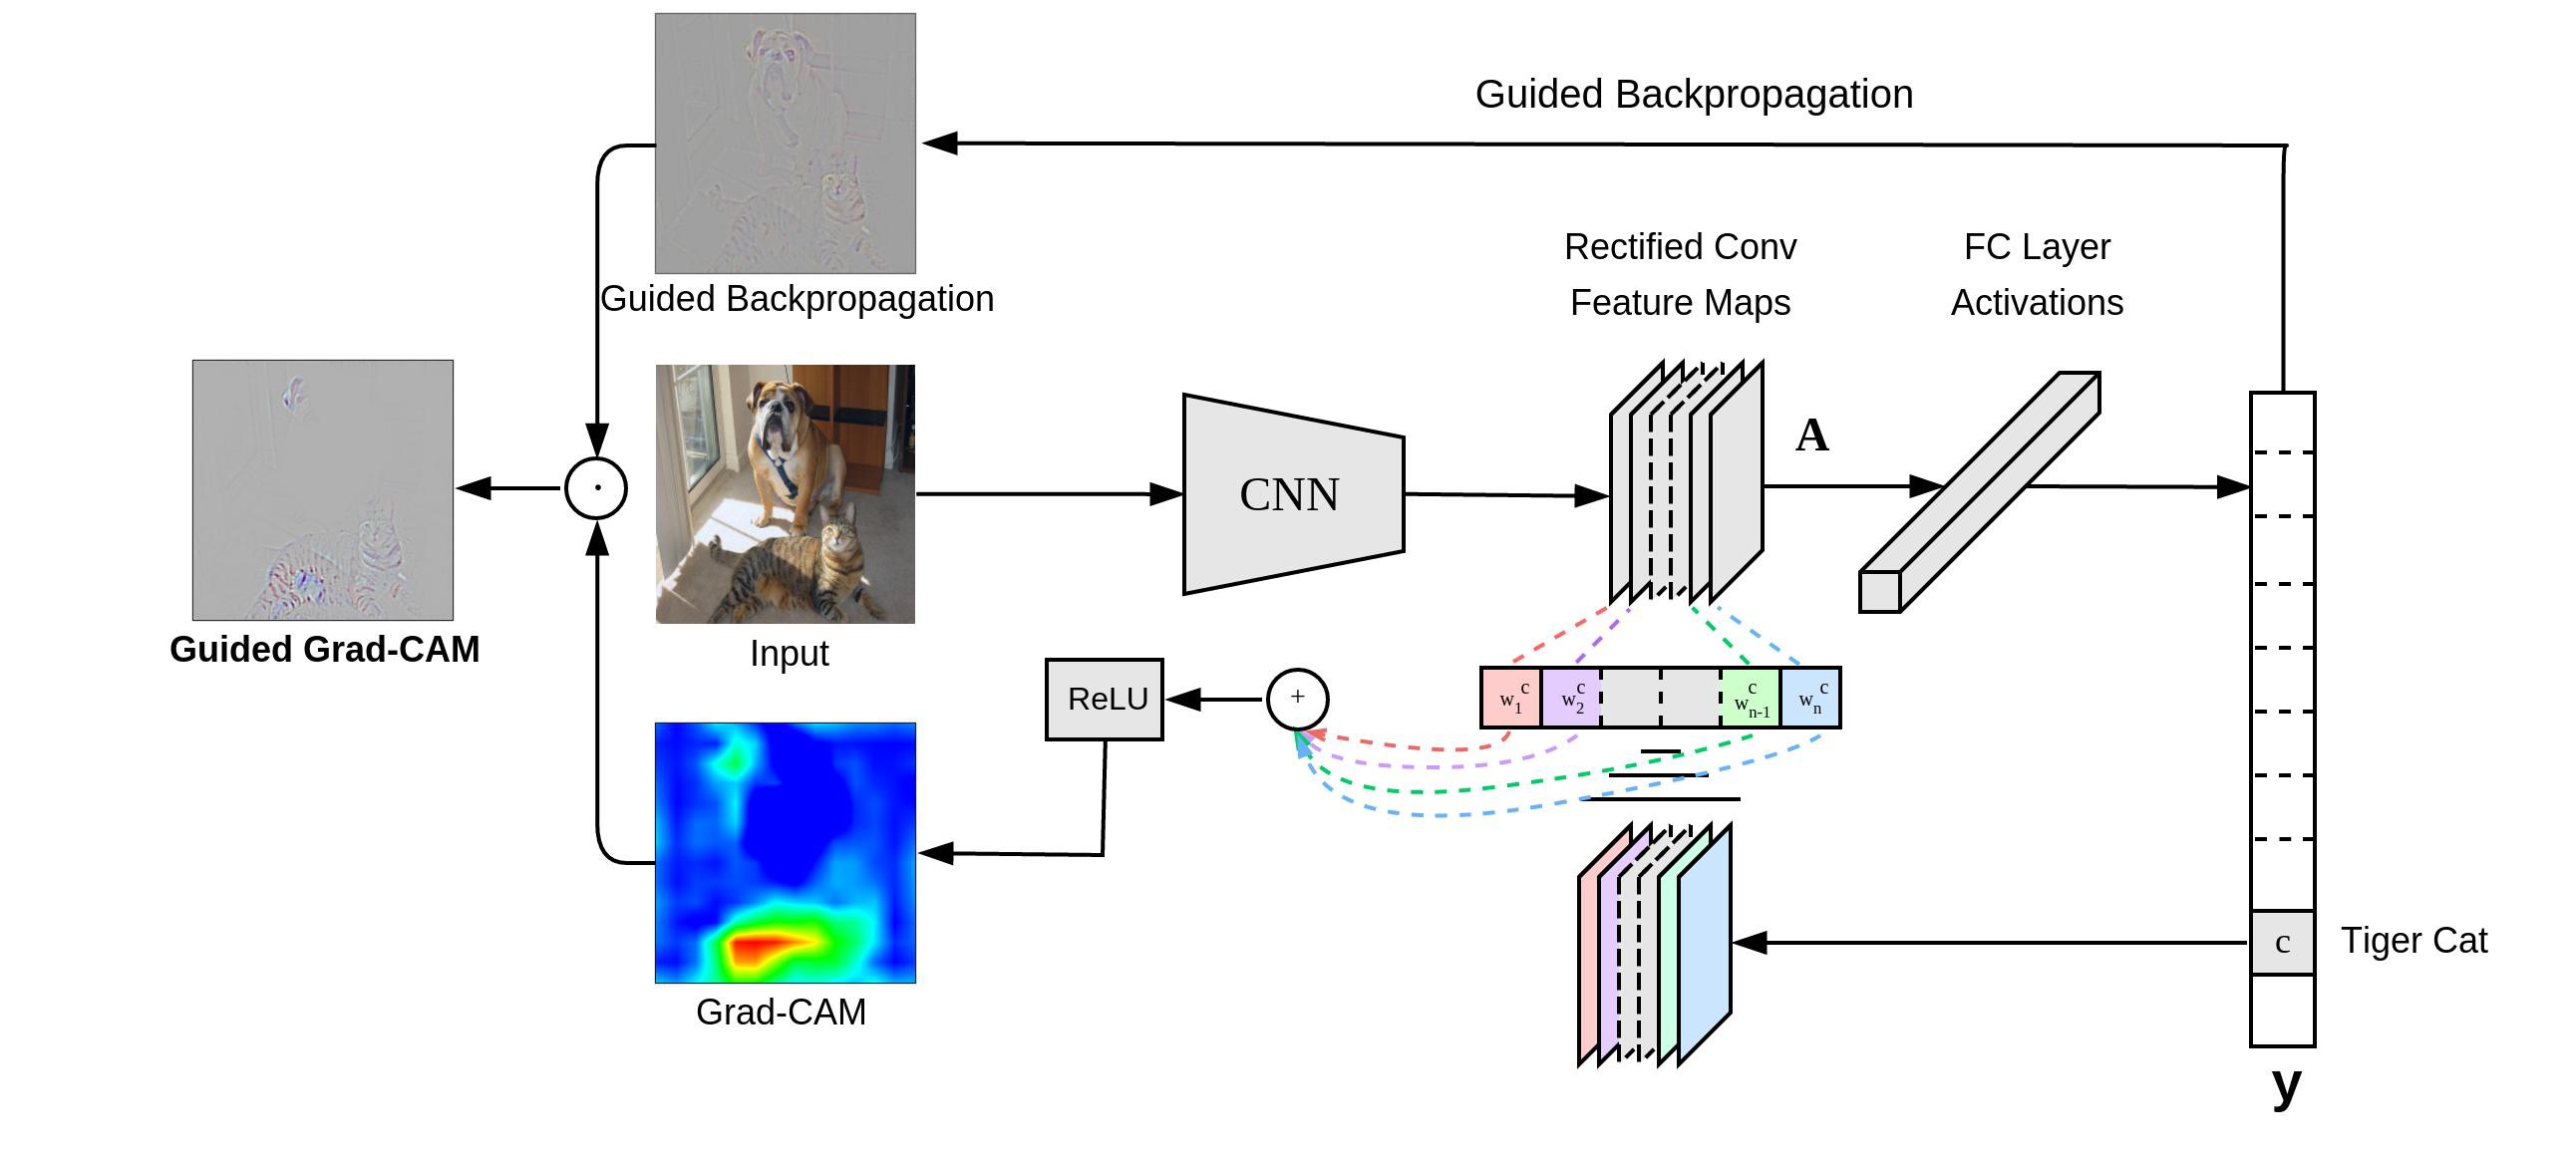
\includegraphics[width=400]{figures/grad_cam_arch.jpeg}
    \caption{Schema of the GradCam algorithm taken from the paper\cite{grad_cam_2019}}
    \label{fig:grad_cam_arch}
\end{figure}

When model goal is to performs multi-class classification it makes sense to apply a relu function to the activation map in order to remove the negative value that could be explaining any other classes in the image. In our case as we are dealing with a binary classification task, it might make sense not to remove negative value and let a clinician decide which map is more useful for him.

The output size of the layer one tries to explain will determines the granularity of the activation map. The artifact due to shrinkage of the network can be seen on figure \ref{fig:grad_cam_multilayer}. This impose a trade off when constructing your model as you don’t want your last convolution layer to be too small in order to keep a good focused explanation. On the other hand if you keep it too big you end up with a too big model for which a lot of data is needed to be trained.

Guided backpropagation\cite{guided_backprop_springenberg2014striving} is another visualization to explain what a model has learnt. Compare to grad-cam it gives a sharper explanation map, but fails at giving an explanation for a specific class. To get the best of both, it is possible to multiply point wise the two outputs as illustrated on the left side of figure \ref{fig:grad_cam_arch}.


\subsection{FullGrad}

Devoloped by Sriniva at EPFL, FullGrad\cite{fullgradient} introduce the a new tool for neural network interpretability that satisfy both \textit{completeness} and \textit{weak dependence on inputs}. Completeness can be seens as the property that the saliency map contains all the information necessary to compute the output of the model.

\begin{figure}
    \centering
    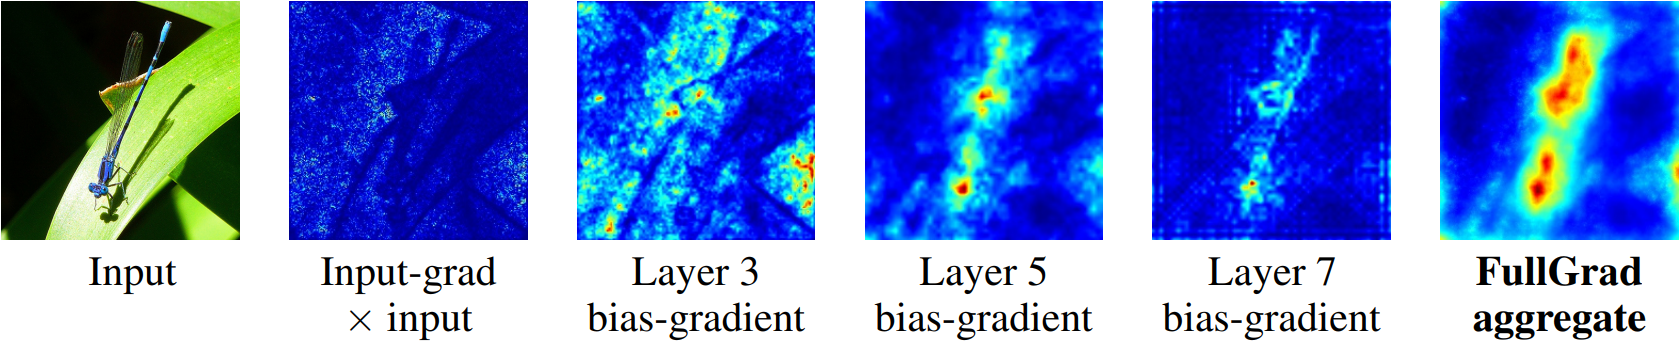
\includegraphics[width=400]{figures/fullgrad_layer_agregation.png}
    \caption[FullGradExample]{Visualization\cite{fullgradient} of bias-gradient at different layer and the output of fullGrad which is an aggregation of the input-gradient and all the intermediate layers.}
    \label{fig:full_grad_layer_aggreagtion}
\end{figure}

A saliency map is complete if there exist a function $\phi$ such that:

$$\phi(S(x), x) = f(x) \text{ } \forall x,f$$

Weak dependence on inputs on the other hand, is a property that you get when slightly changing an important pixel drastically affect the output of the model. Previous methods were not able to have those two property at the same time.

As visualized in figure \ref{fig:full_grad_layer_aggreagtion} the output of the fullGrad algorithm is an aggregation of the gradient at multiple layer. Therefore compare to GradCam there is no need to define a layer of interest which usually is set to the last convolutional layer. This also make the algorithm less sensitive to the potentially small size of the last convolutional layer.